\documentclass[aspectratio=169]{beamer}

\usepackage[T1]{fontenc}
\usepackage{amsmath}
\usepackage{booktabs}
\usepackage{graphicx}
\usepackage{hyperref}
\usepackage{HKUSTstyle}
\usefonttheme{serif}

\graphicspath{{pic/}{pic/psa_ga/}}

\author{Your Name}
\title{Surrogate-Assisted Genetic Optimization of a PSA Process}
\subtitle{\texorpdfstring{Manifest-only CO$_2$ capture optimization with NSGA-II}{Manifest-only CO2 capture optimization with NSGA-II}}
\institute{
    @connect.hkust-gz.edu.cn\\
    SEEN5320 Final Project\\
    The Hong Kong University of Science and Technology (Guangzhou)
}
\date{\small \today}

\begin{document}

\begin{frame}
    \titlepage
    \vspace*{-0.5cm}
    \begin{center}
        
\includegraphics[keepaspectratio,scale=0.025]{UST.png}
    \end{center}
\end{frame}

\begin{frame}{Project Route}
\begin{block}{Goal}
Build a closed surrogate-assisted optimization workflow using only \texttt{data/manifest.csv}.
\end{block}
\begin{itemize}
    \item Removed dependency: deleted time-space CSV files and derived features.
    \item Surrogate inputs: seven PSA operating variables $x_1$--$x_7$.
    \item Surrogate outputs: purity, recovery, productivity, and specific energy.
    \item Optimizer: NSGA-II genetic algorithm coupled to the surrogate.
    \item Closed loop: export optimized inputs for detailed-model reruns and compare returned outputs.
\end{itemize}
\end{frame}

\begin{frame}{Manifest Dataset}
\begin{columns}[T,onlytextwidth]
\begin{column}{0.45\textwidth}
\begin{table}
\centering
\scriptsize
\begin{tabular}{ll}
\toprule
Item & Value \\
\midrule
Successful simulations & 1000 \\
Design variables & 7 \\
KPI outputs & 4 \\
Derived time-space features & 0 \\
Train/test split & 80/20 \\
\bottomrule
\end{tabular}
\end{table}
\begin{itemize}
    \item Bounds are read from \texttt{ProcessConfig.yaml}.
    \item Energy is modeled in log space because it is highly skewed.
\end{itemize}
\end{column}
\begin{column}{0.52\textwidth}
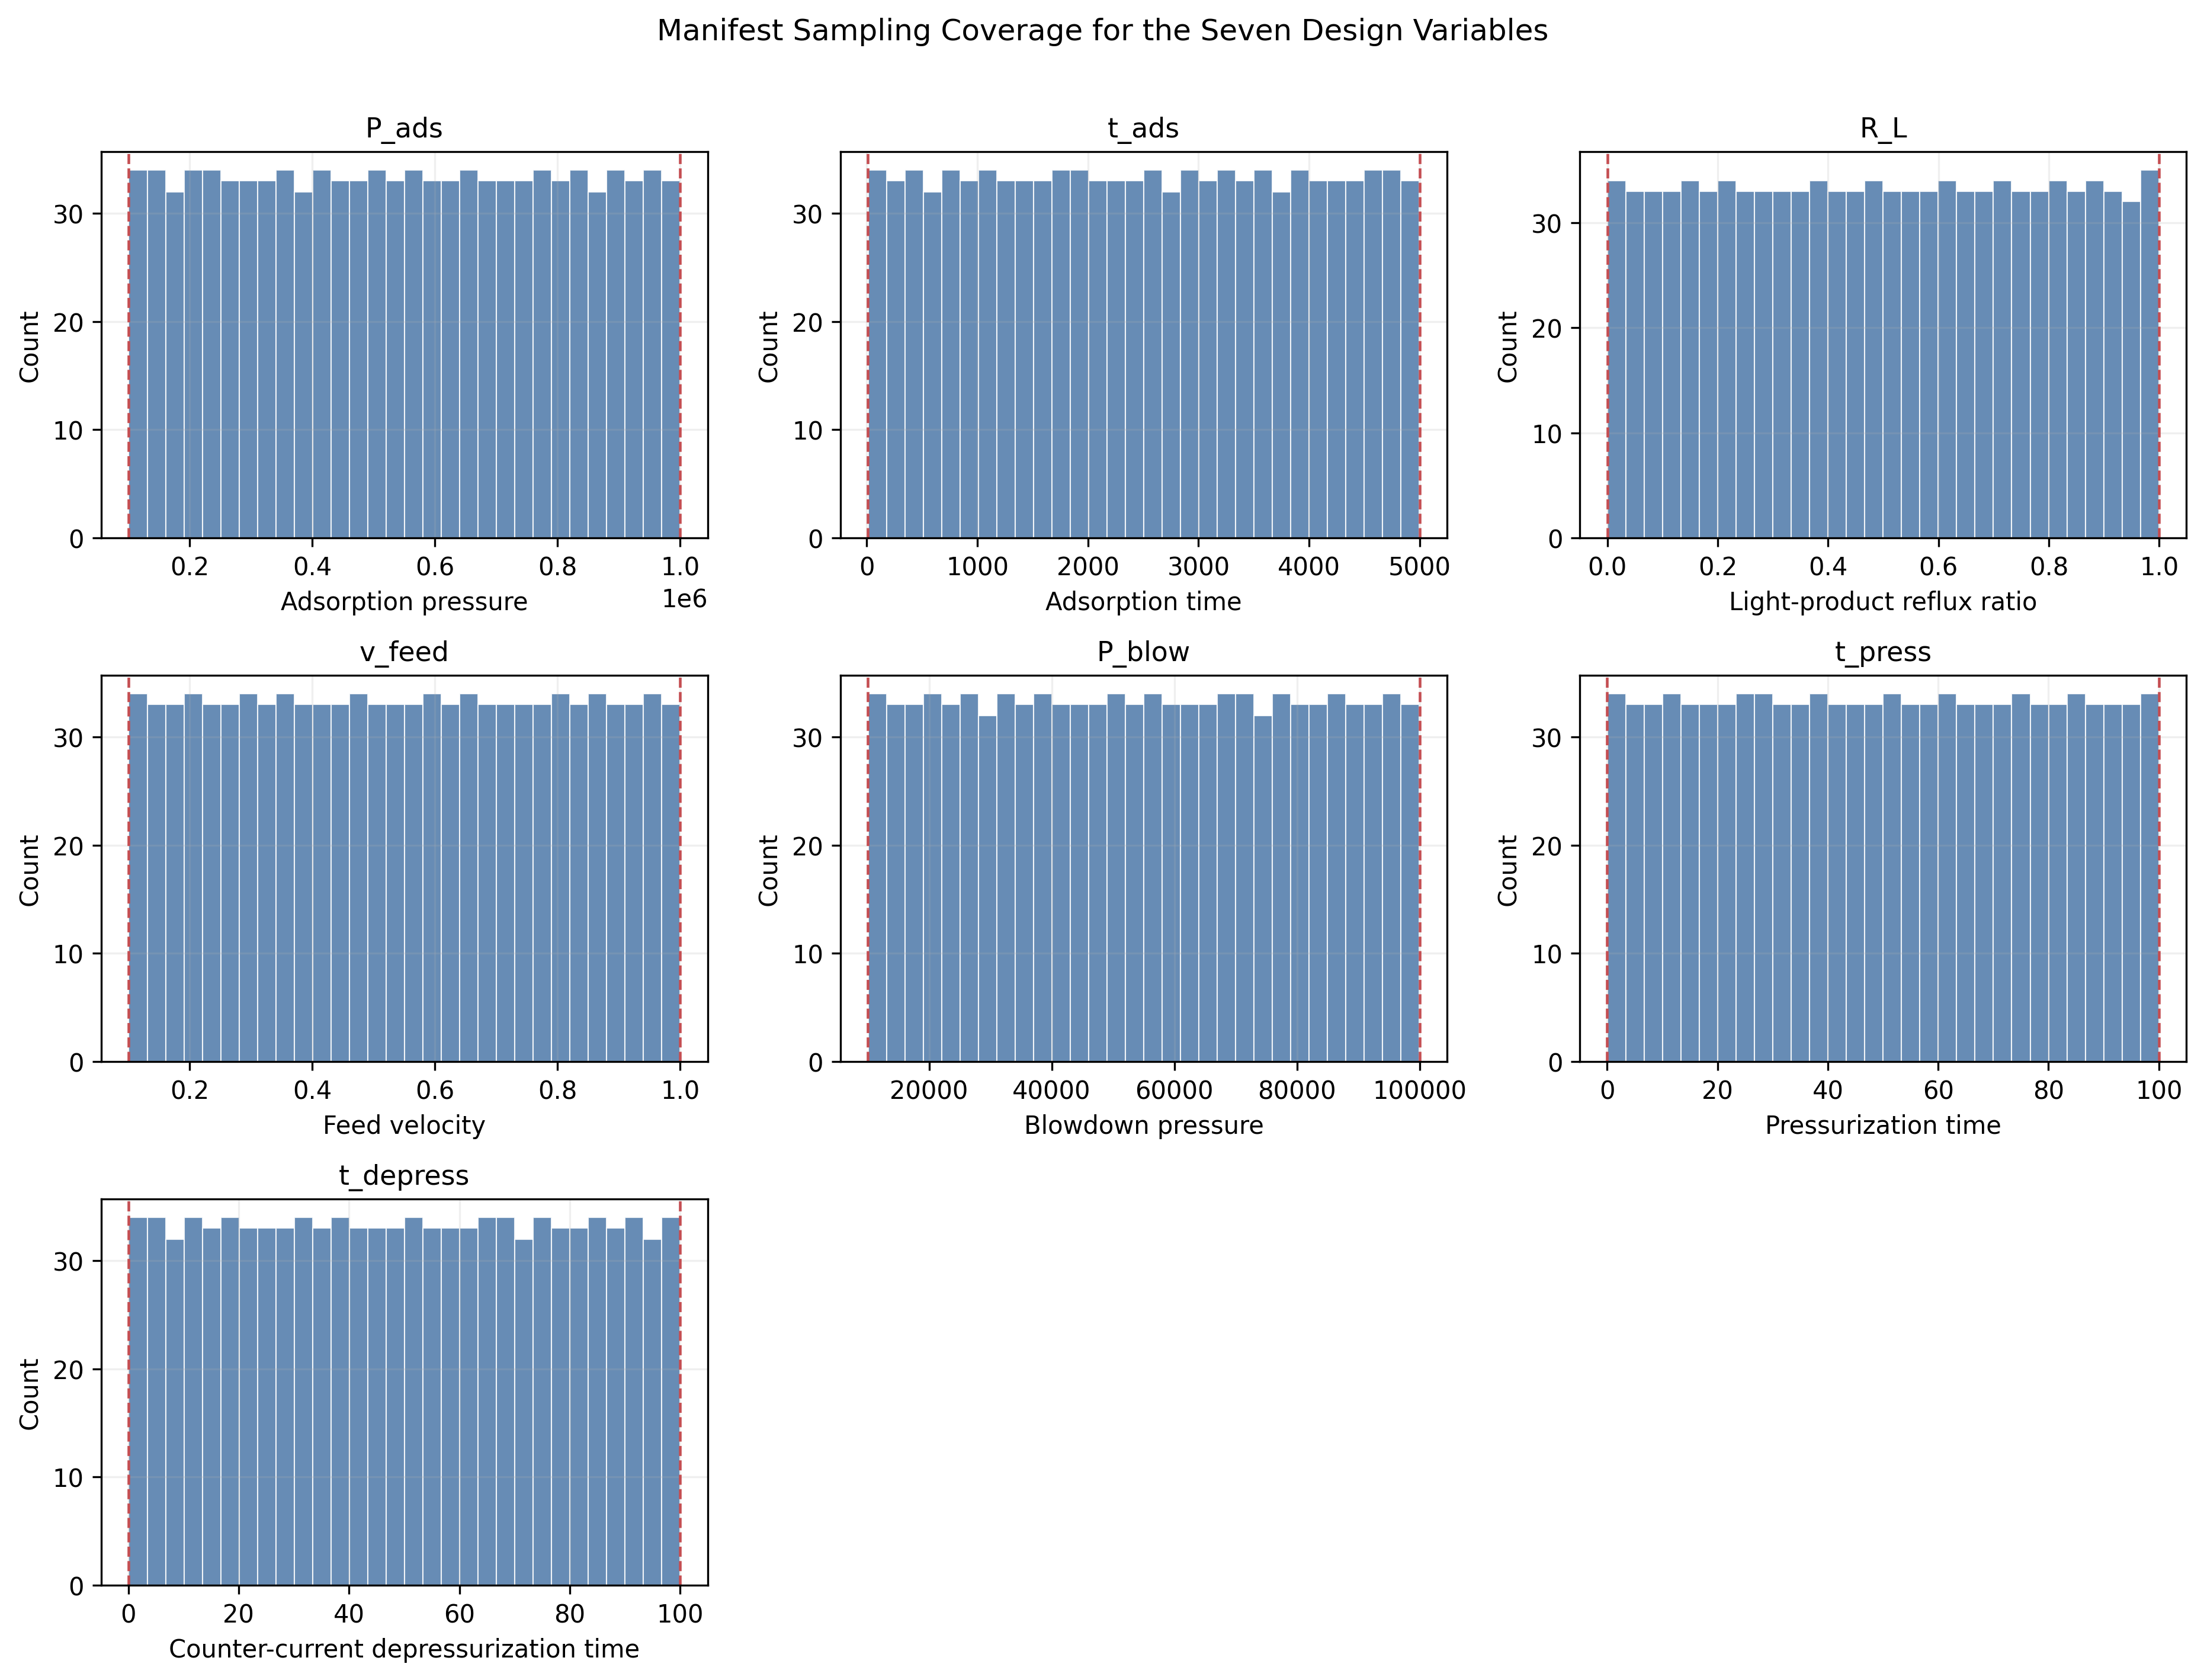
\includegraphics[width=\textwidth]{01_manifest_sampling_coverage.png}
\end{column}
\end{columns}
\end{frame}

\begin{frame}{Surrogate Model}
\begin{columns}[T,onlytextwidth]
\begin{column}{0.46\textwidth}
\begin{itemize}
    \item Degree-3 ridge response surface in standardized design variables.
    \item Purity target: $\log_{10}(purity - 0.15)$.
    \item Other targets: recovery, productivity, and $\log_{10}(energy)$.
    \item Ridge regularization selected by five-fold cross-validation.
    \item Output predictions clipped to the observed manifest range before GA search.
\end{itemize}
\end{column}
\begin{column}{0.52\textwidth}
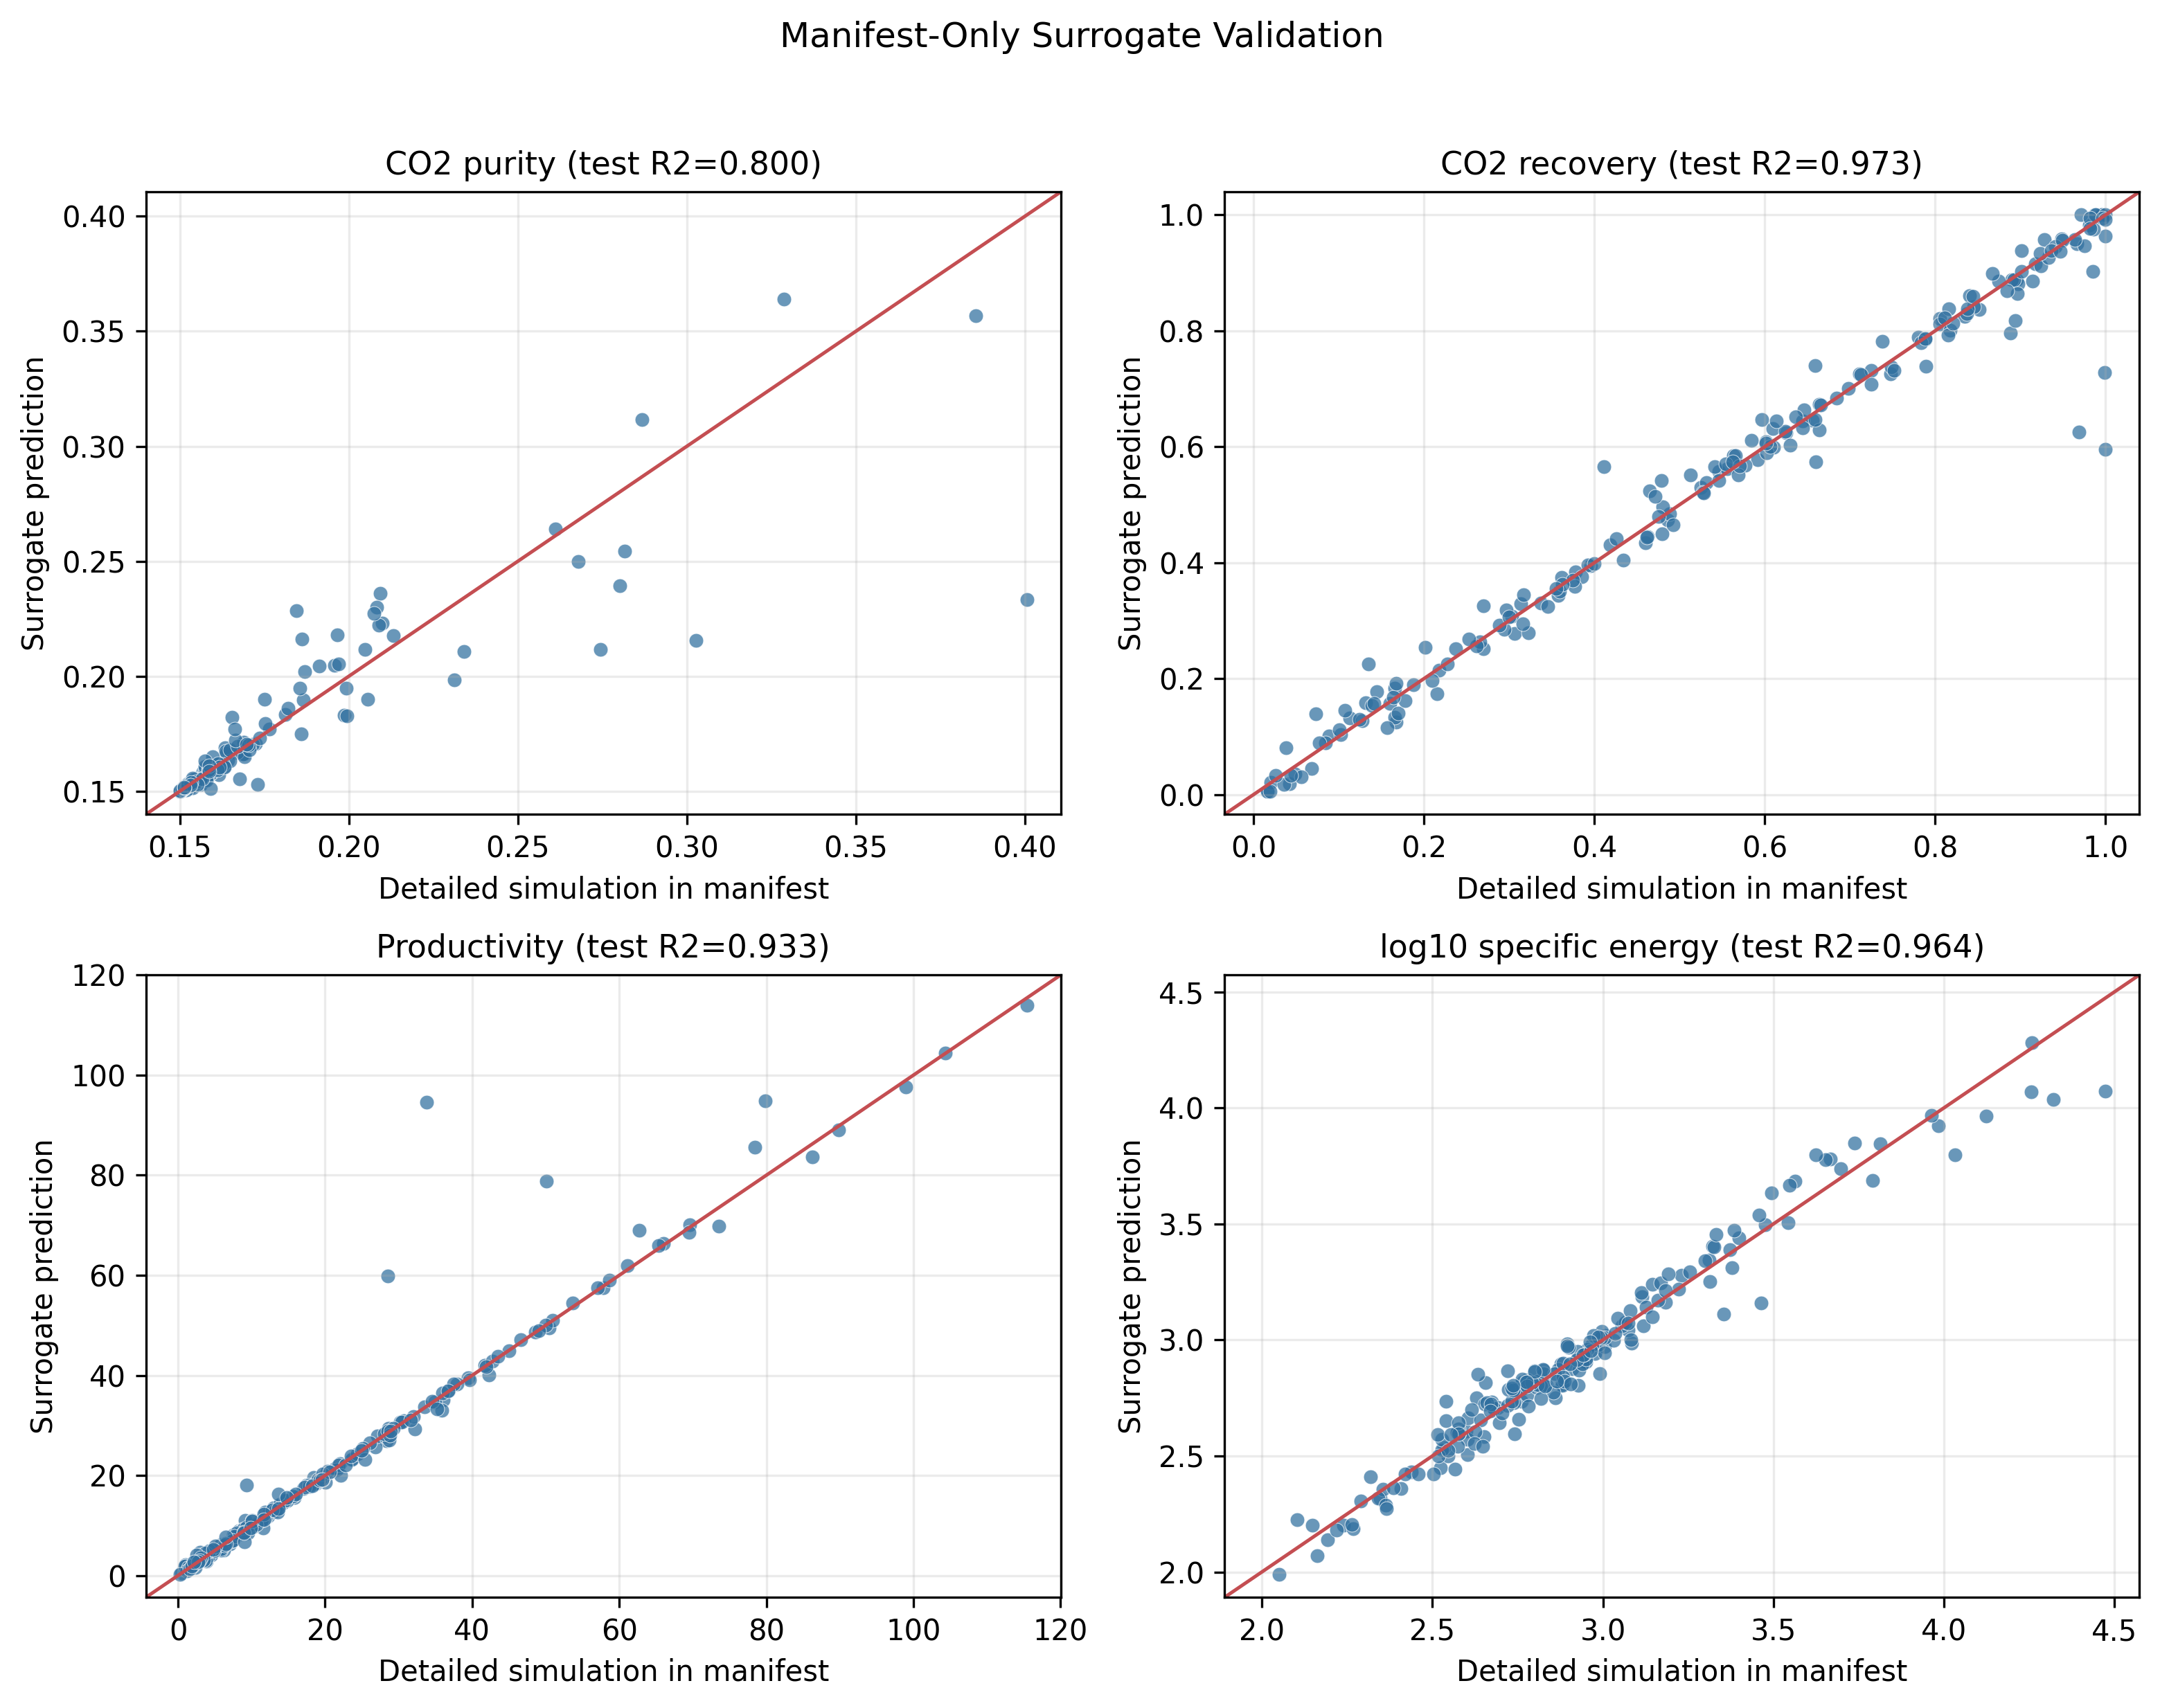
\includegraphics[width=\textwidth]{02_surrogate_validation.png}
\end{column}
\end{columns}
\end{frame}

\begin{frame}{Surrogate Accuracy}
\begin{columns}[T,onlytextwidth]
\begin{column}{0.48\textwidth}
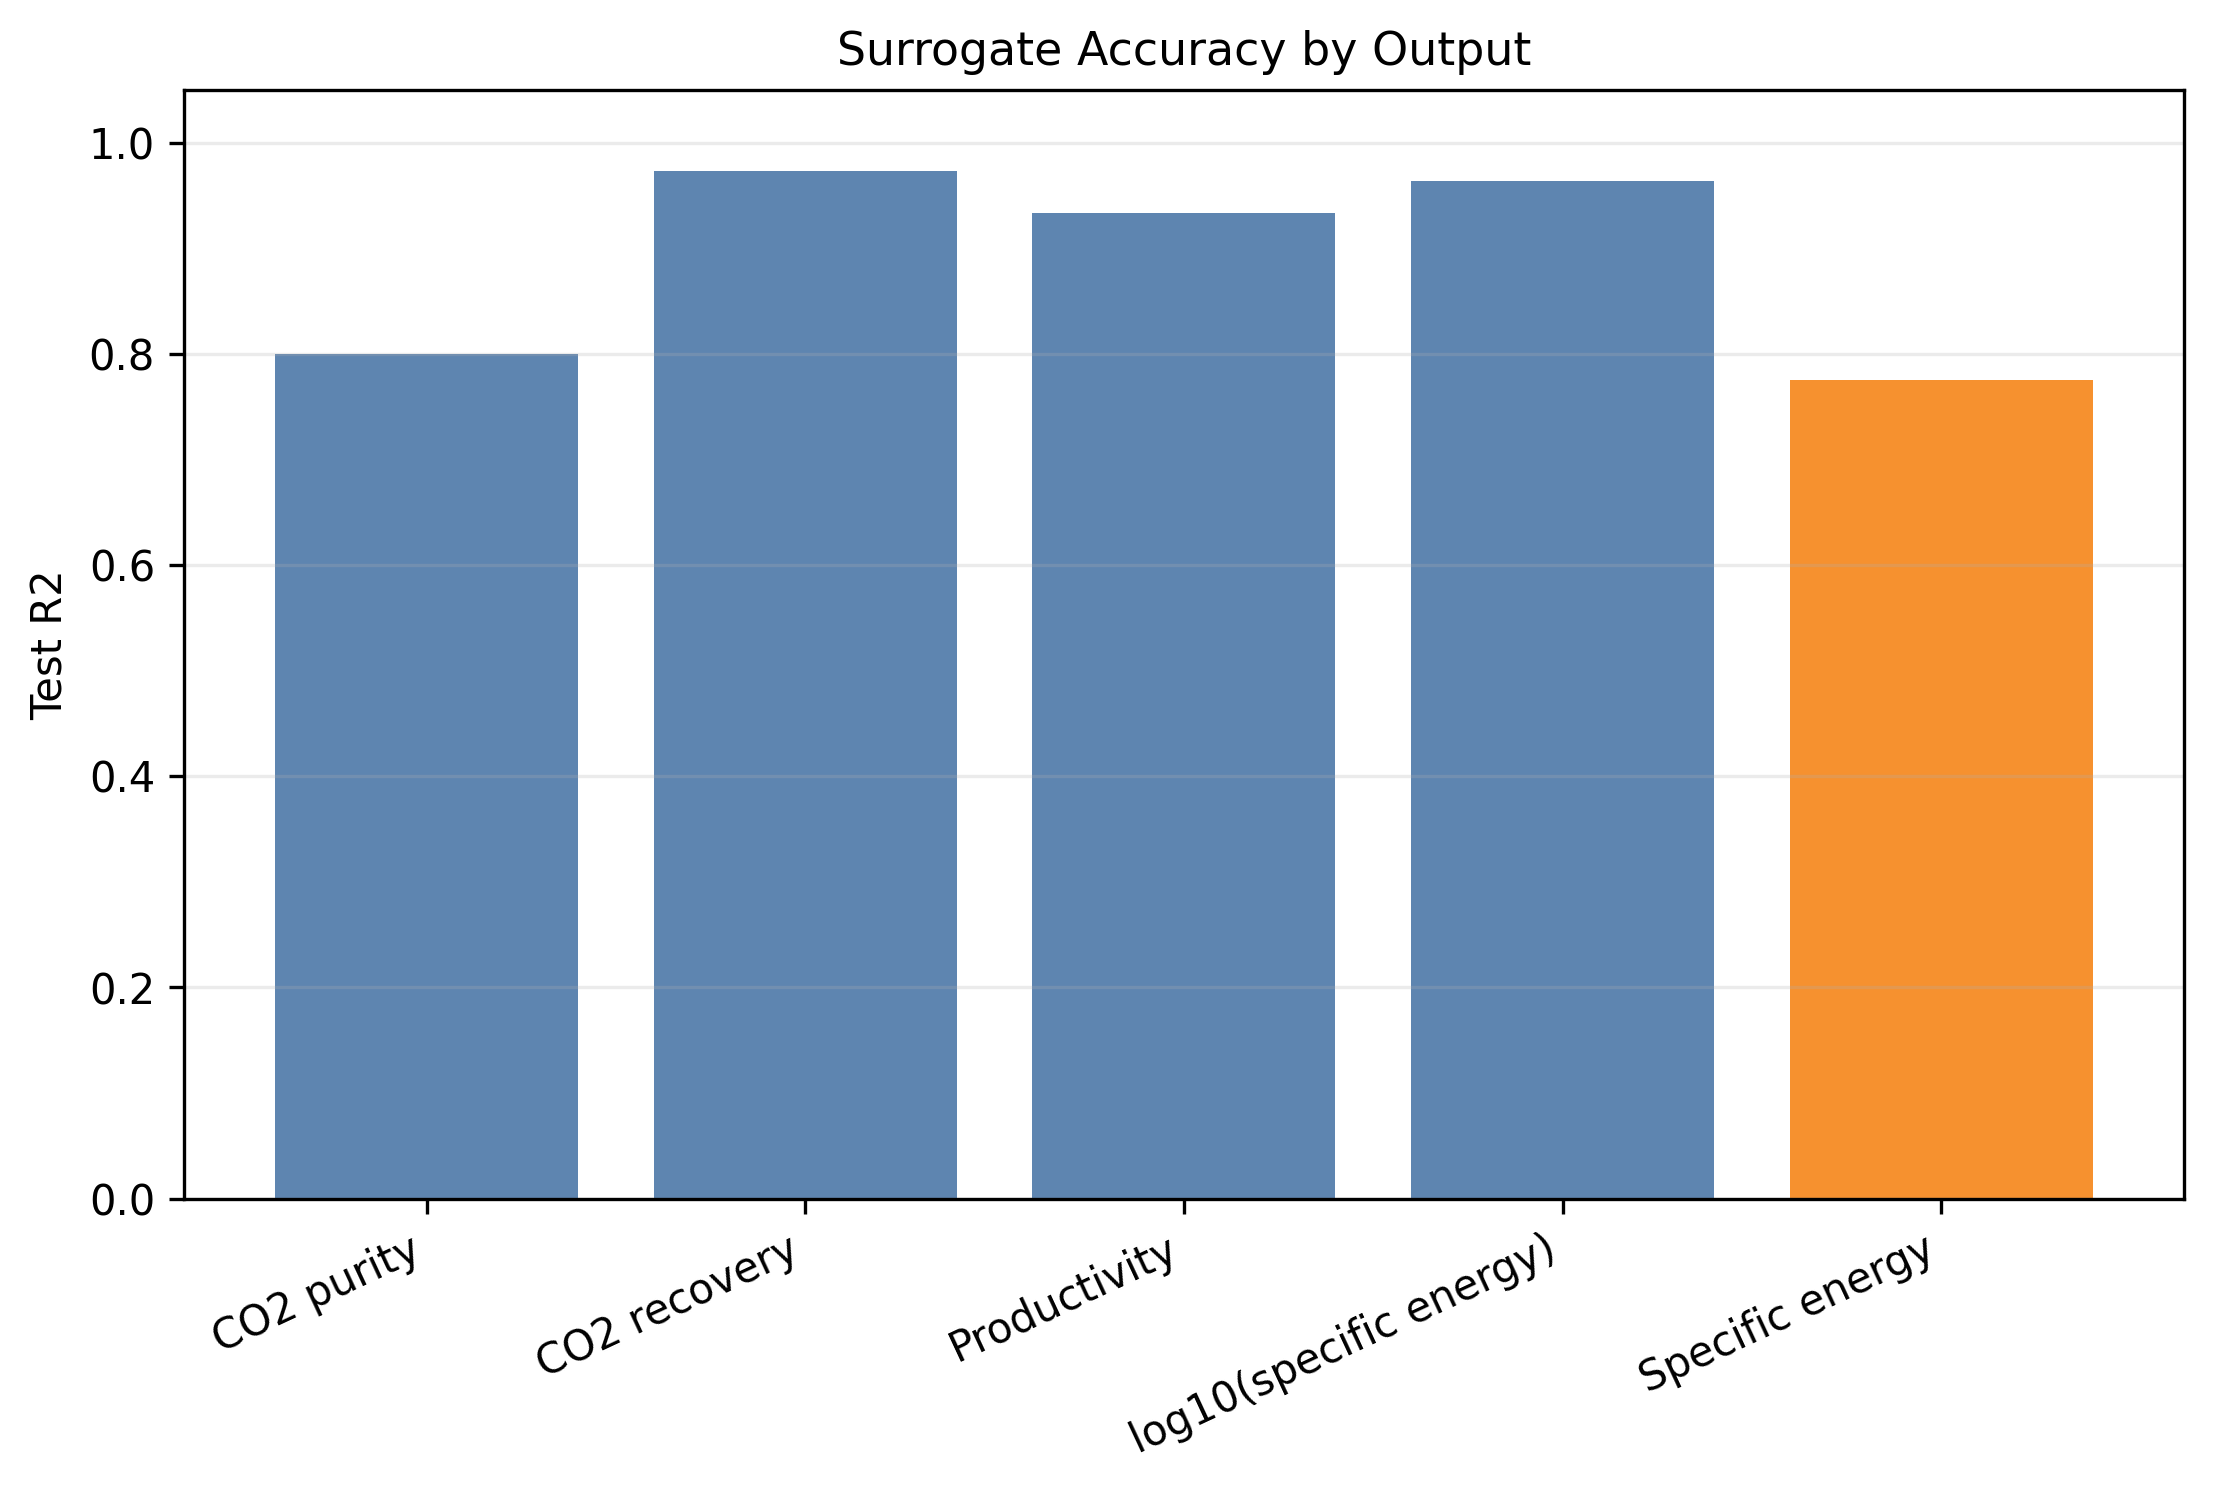
\includegraphics[width=\textwidth]{03_surrogate_metric_summary.png}
\end{column}
\begin{column}{0.49\textwidth}
\begin{table}
\centering
\scriptsize
\begin{tabular}{lcc}
\toprule
Target & RMSE & Test $R^2$ \\
\midrule
Purity & 0.0166 & 0.800 \\
Recovery & 0.0502 & 0.973 \\
Productivity & 5.50 & 0.933 \\
$\log_{10}$(energy) & 0.0817 & 0.964 \\
\bottomrule
\end{tabular}
\end{table}
\begin{itemize}
    \item Purity is the hardest scalar-output target.
    \item Recovery, productivity, and log-energy are reliable enough for screening.
\end{itemize}
\end{column}
\end{columns}
\end{frame}

\begin{frame}{GA Optimization Setup}
\begin{columns}[T,onlytextwidth]
\begin{column}{0.48\textwidth}
\textbf{NSGA-II settings}
\begin{itemize}
    \item Population size: 120.
    \item Generations: 200.
    \item Simulated binary crossover: 0.9.
    \item Polynomial mutation: $1/7$ per variable.
    \item Initial population: manifest-seeded plus random points.
\end{itemize}
\end{column}
\begin{column}{0.48\textwidth}
\textbf{Two bi-objective fronts}
\begin{itemize}
    \item Maximize purity and recovery.
    \item Maximize productivity and minimize energy.
    \item Export 20 representative candidates per front for detailed-model reruns.
\end{itemize}
\end{column}
\end{columns}
\end{frame}

\begin{frame}{Front 1: Purity vs Recovery}
\begin{columns}[T,onlytextwidth]
\begin{column}{0.58\textwidth}
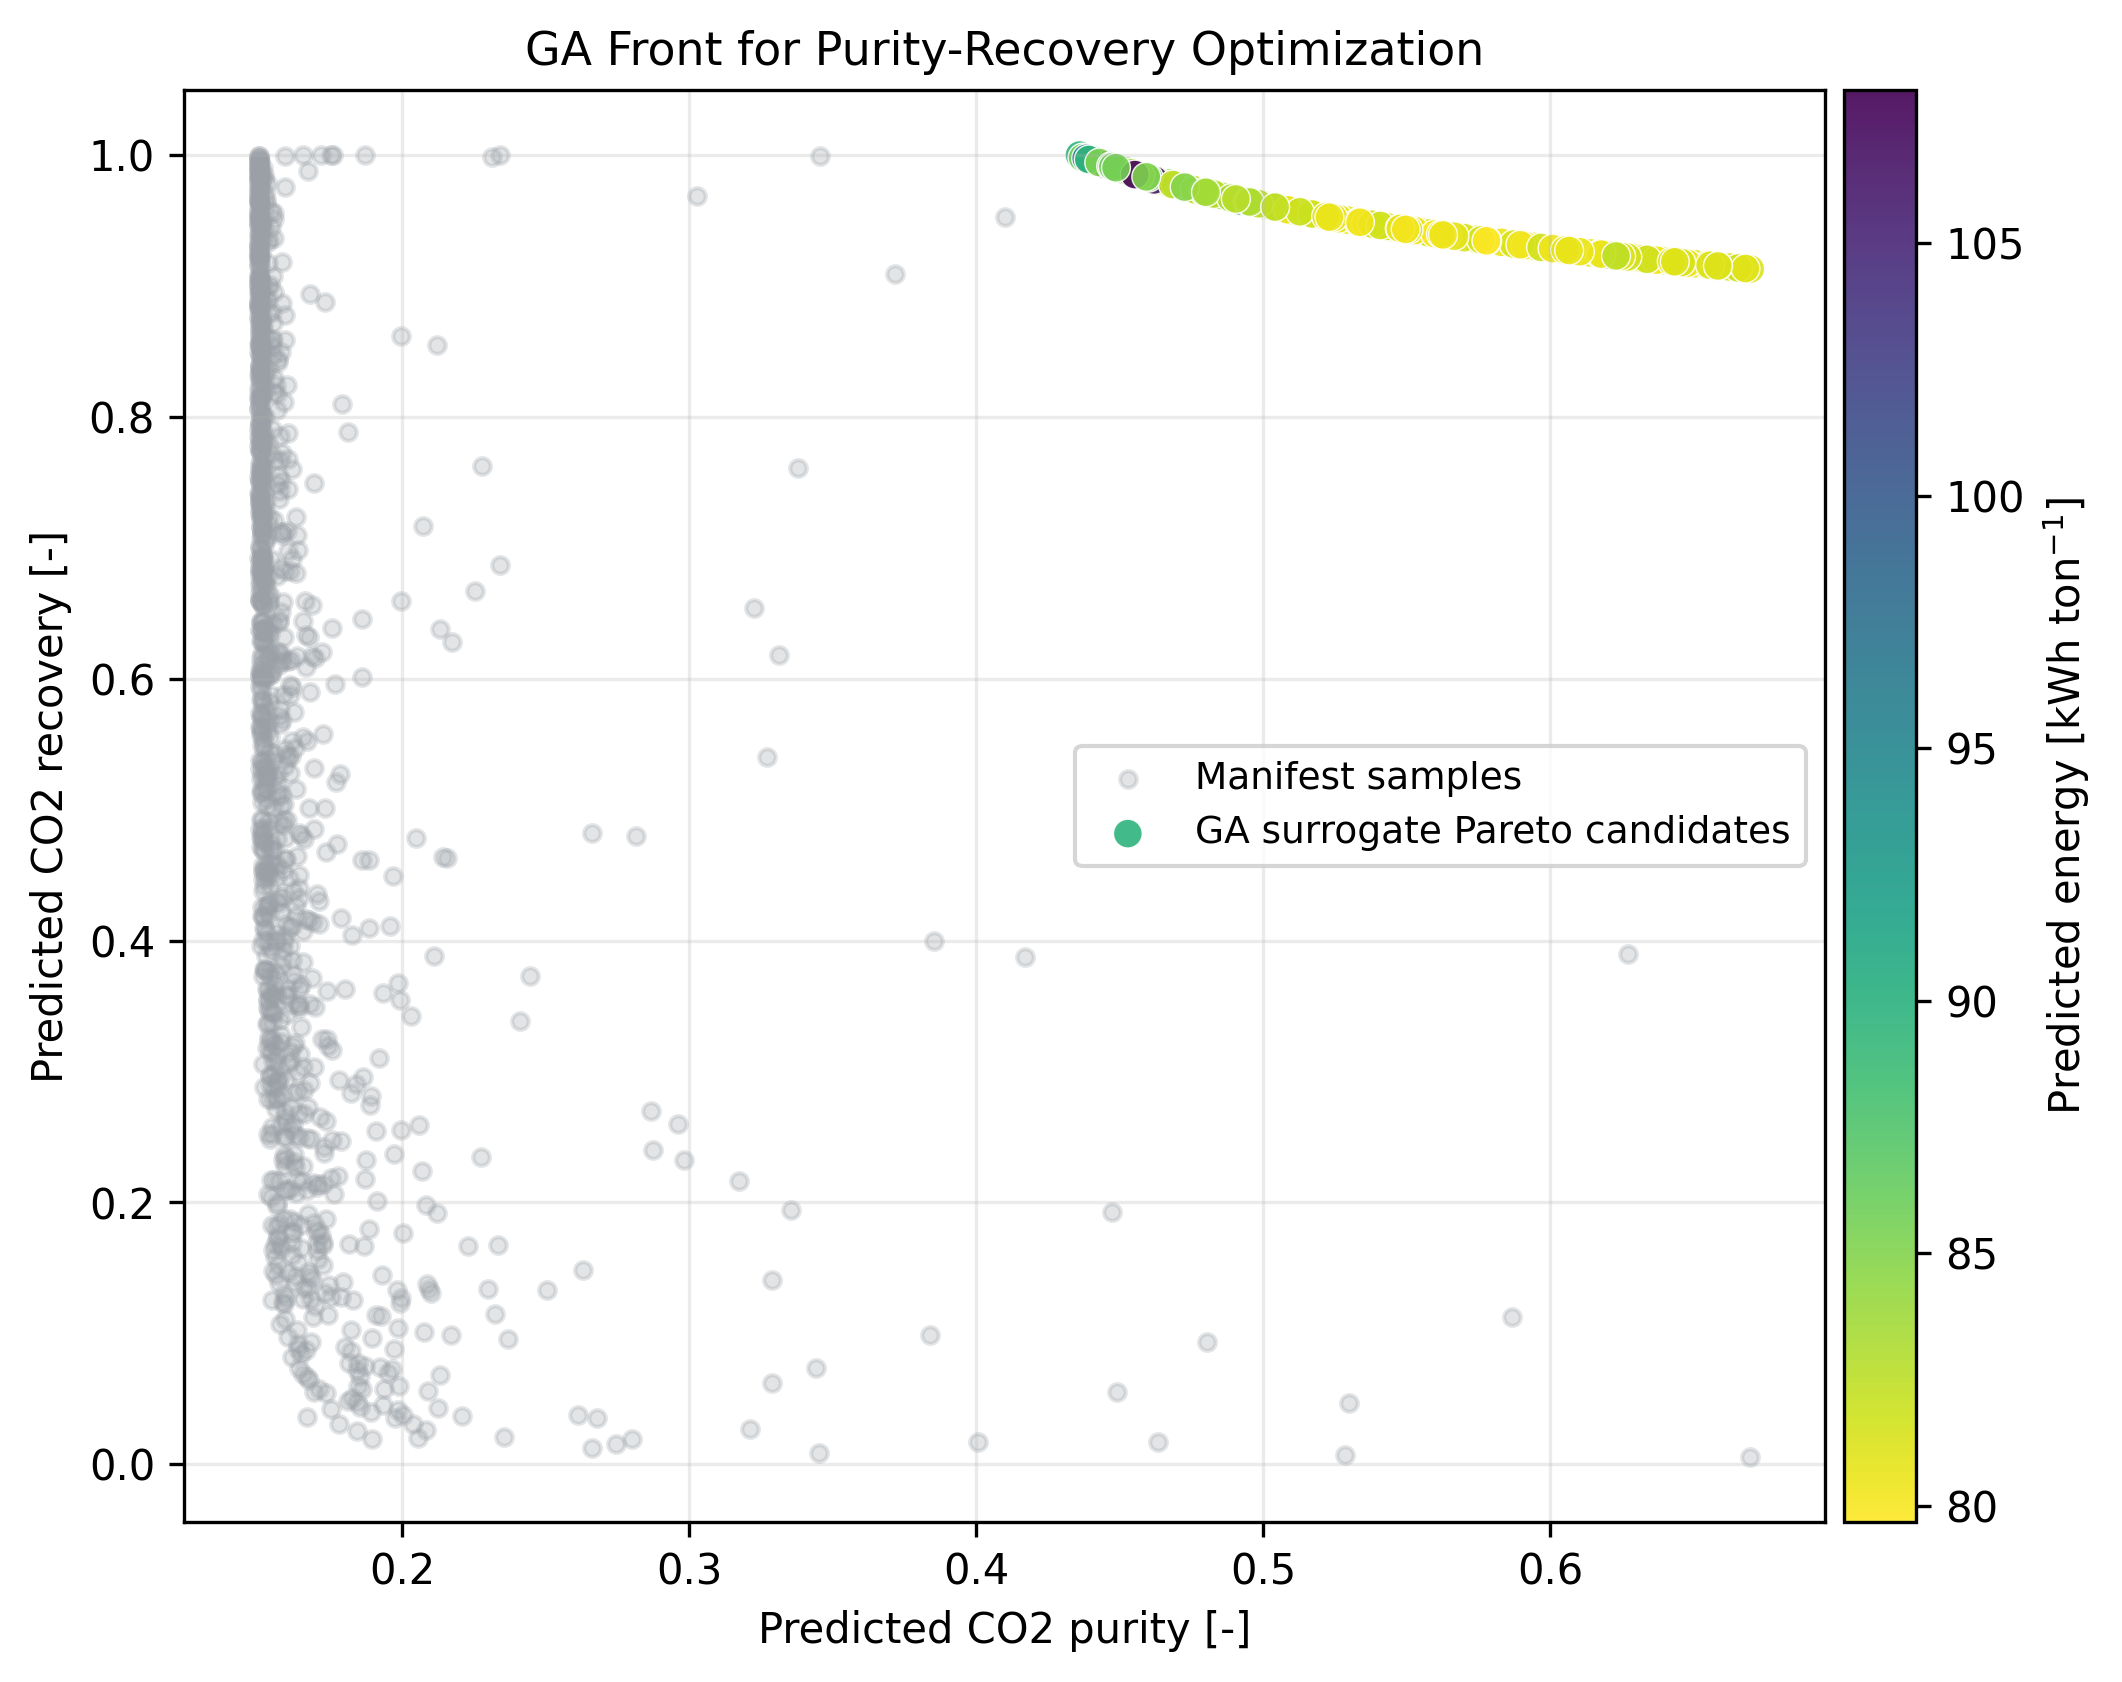
\includegraphics[width=\textwidth]{04_ga_purity_recovery_front.png}
\end{column}
\begin{column}{0.39\textwidth}
\begin{itemize}
    \item Predicted purity range: 0.436--0.670.
    \item Predicted recovery range: 0.913--1.000.
    \item Productivity remains low: about 5.5--5.9 mol kg$^{-1}$ h$^{-1}$.
    \item These candidates are separation-quality screening points.
\end{itemize}
\end{column}
\end{columns}
\end{frame}

\begin{frame}{Front 2: Productivity vs Energy}
\begin{columns}[T,onlytextwidth]
\begin{column}{0.58\textwidth}
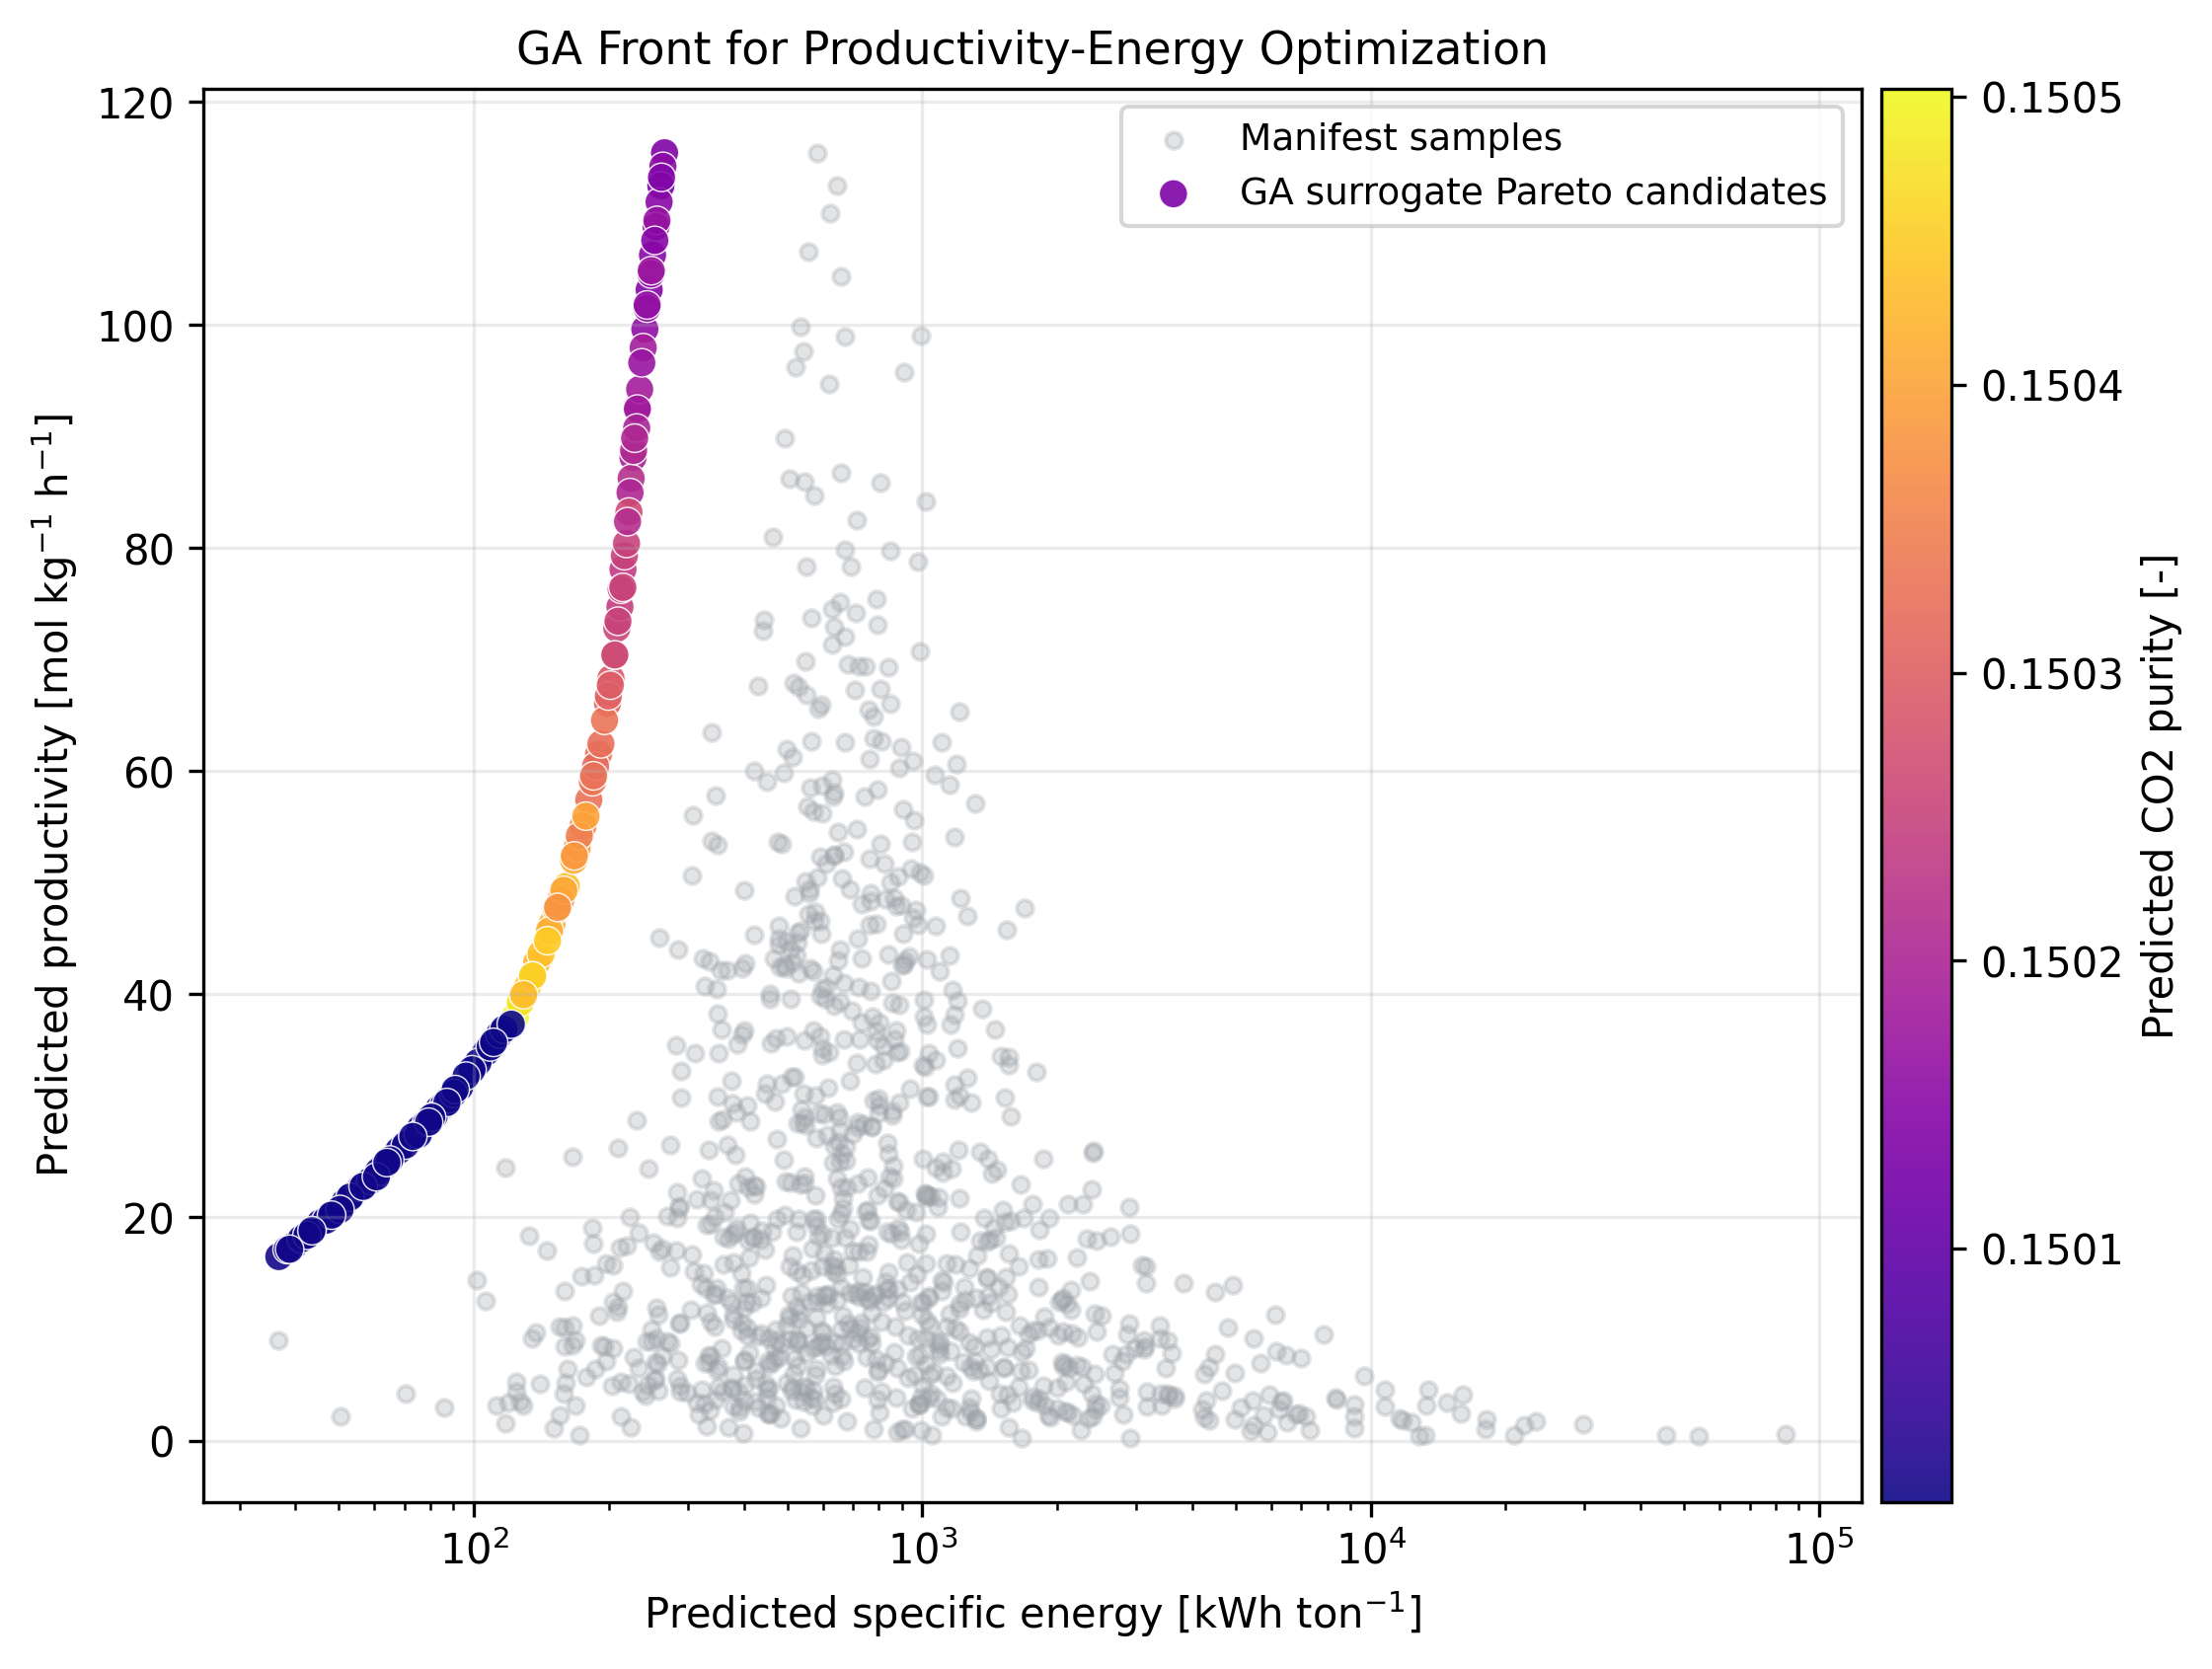
\includegraphics[width=\textwidth]{05_ga_productivity_energy_front.png}
\end{column}
\begin{column}{0.39\textwidth}
\begin{itemize}
    \item Predicted productivity range: 16.49--115.45 mol kg$^{-1}$ h$^{-1}$.
    \item Predicted energy range: 36.70--266.08 kWh ton$^{-1}$.
    \item Purity remains near feed level.
    \item This front is mainly a throughput-energy tradeoff.
\end{itemize}
\end{column}
\end{columns}
\end{frame}

\begin{frame}{Closed-Loop Handoff}
\begin{columns}[T,onlytextwidth]
\begin{column}{0.52\textwidth}
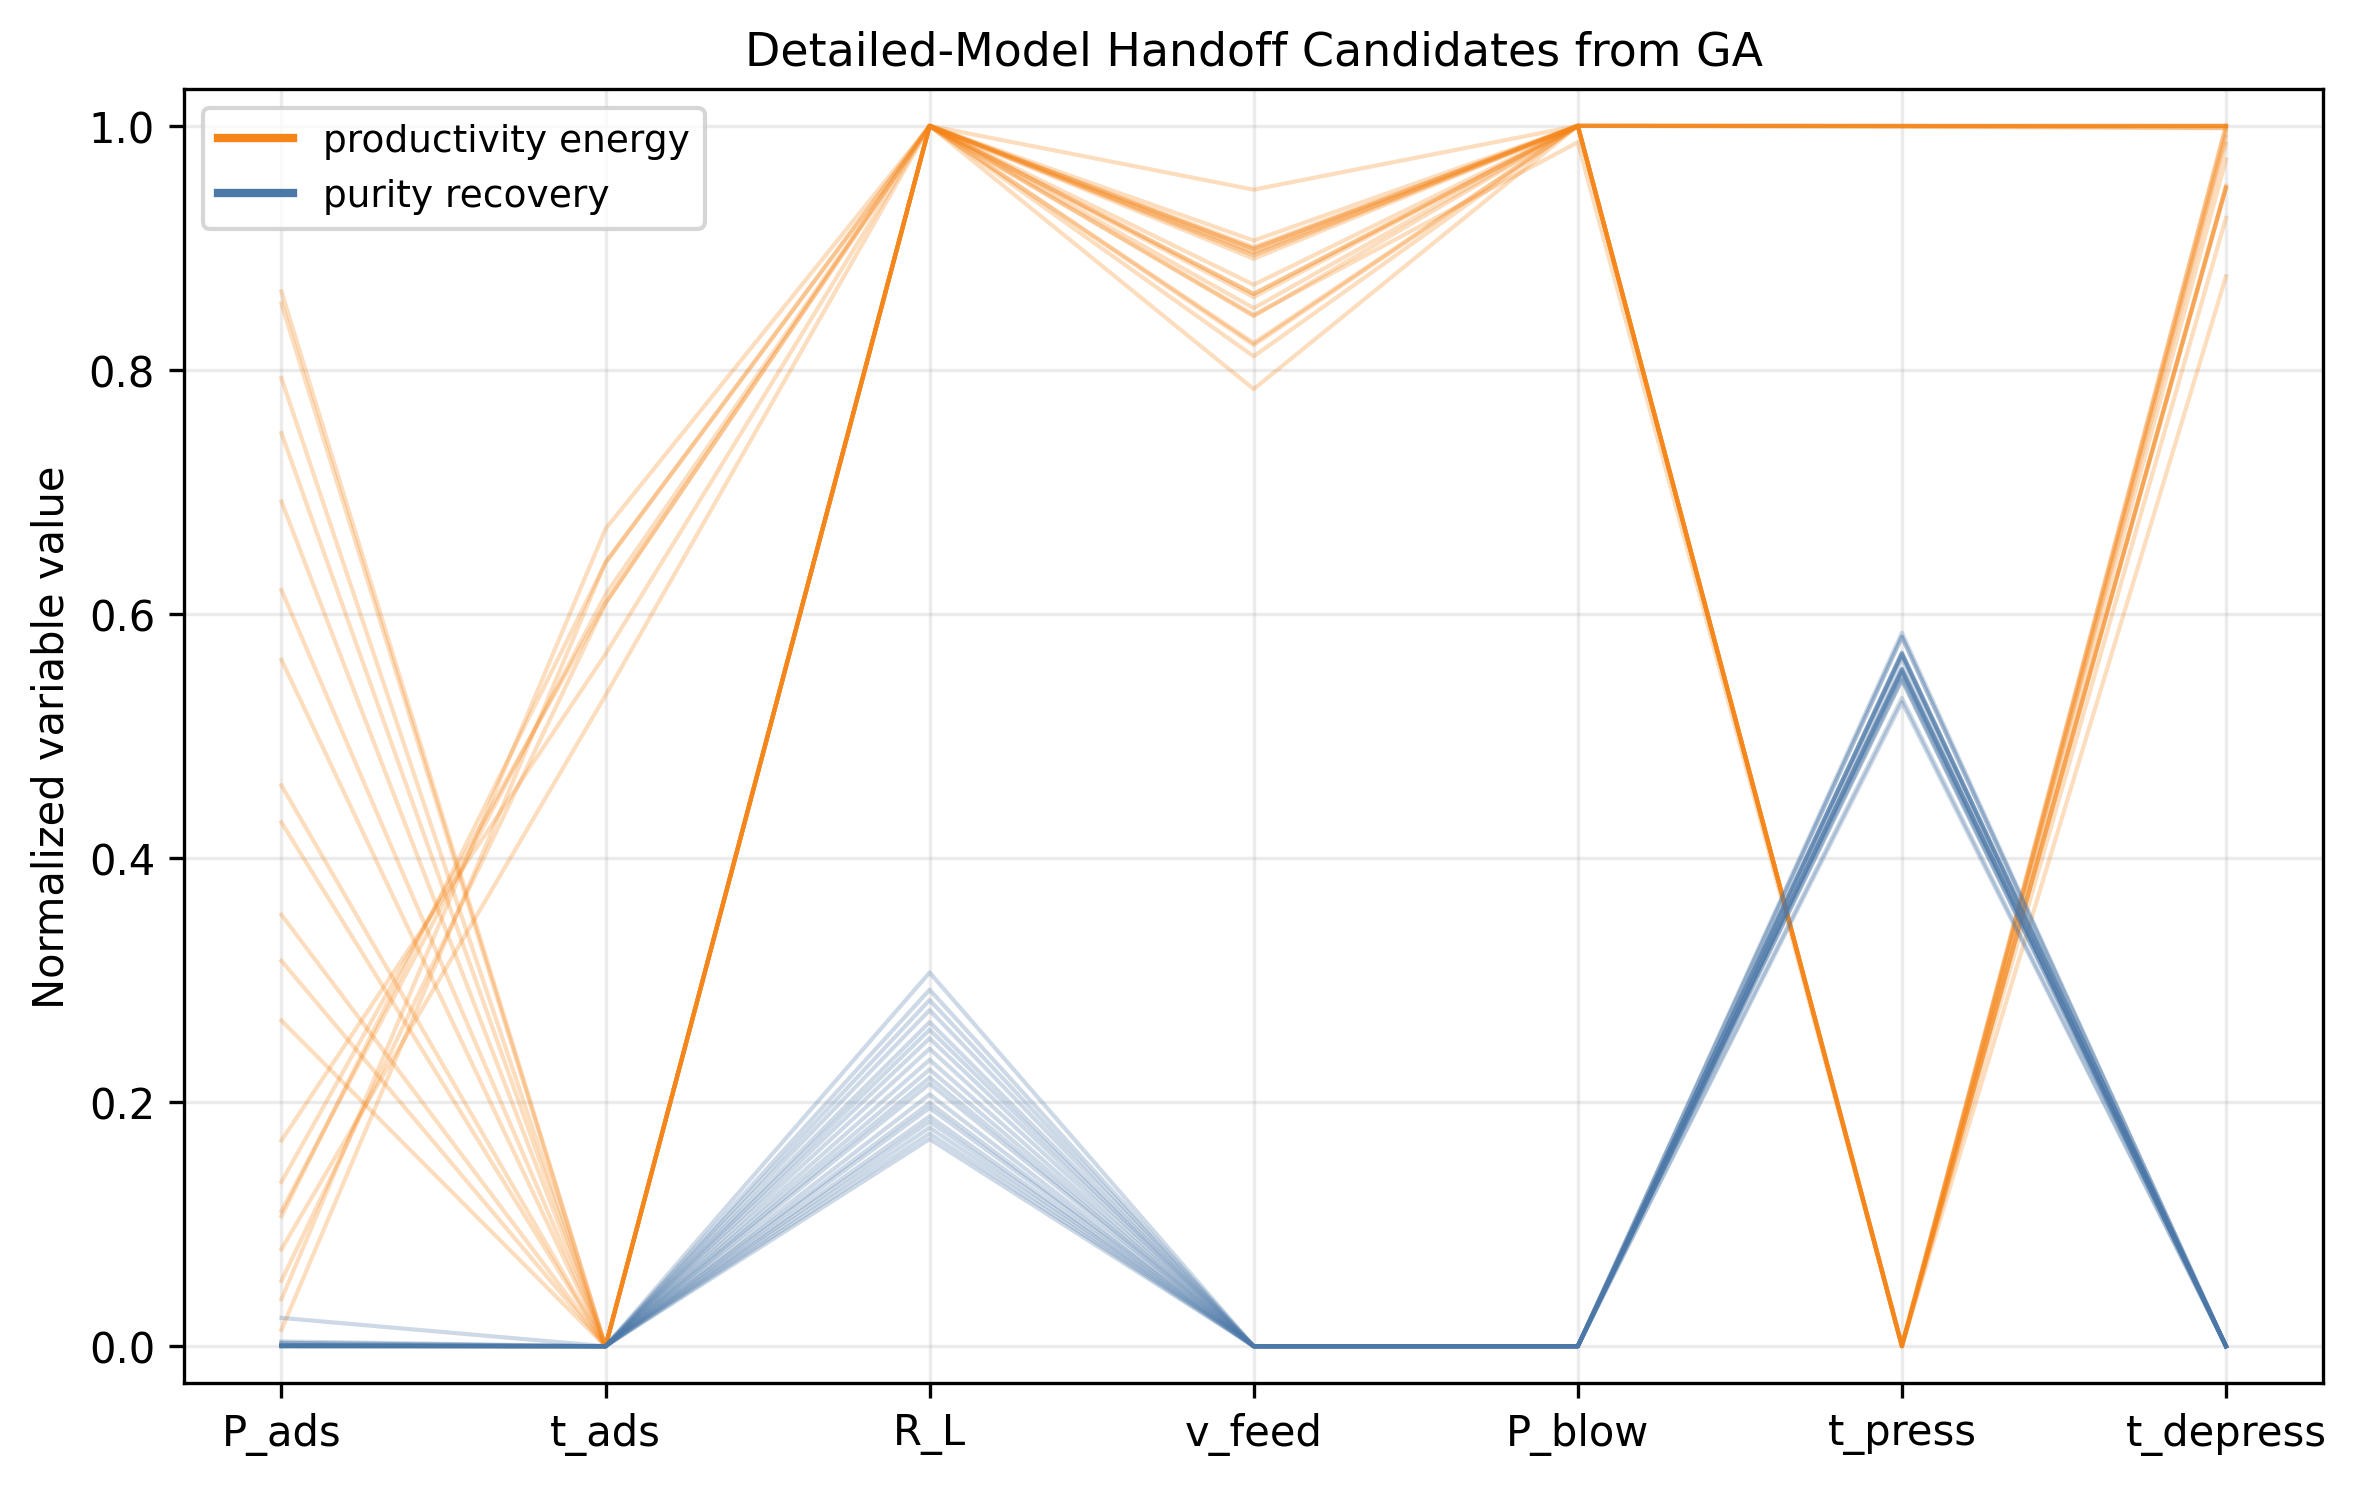
\includegraphics[width=\textwidth]{06_closed_loop_handoff_or_comparison.png}
\end{column}
\begin{column}{0.45\textwidth}
\begin{itemize}
    \item Full final GA populations are saved as CSV.
    \item Surrogate Pareto candidates are saved separately.
    \item Forty rerun inputs are exported for the detailed model.
    \item A result template defines the expected return format.
    \item The comparison script computes errors after detailed results are saved.
\end{itemize}
\end{column}
\end{columns}
\end{frame}

\begin{frame}{Conclusions}
\begin{itemize}
    \item The project now uses only existing manifest data for surrogate training.
    \item NSGA-II turns the surrogate into two explicit multi-objective design fronts.
    \item Output clipping prevents the GA from reporting values outside the manifest training envelope.
    \item Purity-optimized candidates require detailed-model confirmation because purity is the weakest surrogate target.
    \item The CSV handoff completes the closed-loop structure for surrogate-versus-detailed comparison.
\end{itemize}
\end{frame}

\end{document}
